\documentclass[10pt, a5paper]{article}
\usepackage{pdfpages}
\usepackage{parallel}
\usepackage[T2A]{fontenc}
\usepackage{ucs}
\usepackage[utf8x]{inputenc}
\usepackage[polish,english,russian]{babel}
\usepackage{hyperref}
\usepackage{rotating}
\usepackage[inner=2cm,top=1.8cm,outer=2cm,bottom=2.3cm,nohead]{geometry}
\usepackage{listings}
\usepackage{graphicx}
\usepackage{wrapfig}
\usepackage{longtable}
\usepackage{indentfirst}
\usepackage{array}
\newcolumntype{P}[1]{>{\raggedright\arraybackslash}p{#1}}
\frenchspacing
\usepackage{fixltx2e} %text sub- and superscripts
\usepackage{icomma} % коскі ў матэматычным рэжыме
\PreloadUnicodePage{4}

\newcommand{\longpage}{\enlargethispage{\baselineskip}}
\newcommand{\shortpage}{\enlargethispage{-\baselineskip}}

\def\switchlang#1{\expandafter\csname switchlang#1\endcsname}
\def\switchlangbe{
\let\saverefname=\refname%
\def\refname{Літаратура}%
\def\figurename{Іл.}%
}
\def\switchlangen{
\let\saverefname=\refname%
\def\refname{References}%
\def\figurename{Fig.}%
}
\def\switchlangru{
\let\saverefname=\refname%
\let\savefigurename=\figurename%
\def\refname{Литература}%
\def\figurename{Рис.}%
}

\hyphenation{admi-ni-stra-tive}
\hyphenation{ex-pe-ri-ence}
\hyphenation{fle-xi-bi-li-ty}
\hyphenation{Py-thon}
\hyphenation{ma-the-ma-ti-cal}
\hyphenation{re-ported}
\hyphenation{imp-le-menta-tions}
\hyphenation{pro-vides}
\hyphenation{en-gi-neering}
\hyphenation{com-pa-ti-bi-li-ty}
\hyphenation{im-pos-sible}
\hyphenation{desk-top}
\hyphenation{elec-tro-nic}
\hyphenation{com-pa-ny}
\hyphenation{de-ve-lop-ment}
\hyphenation{de-ve-loping}
\hyphenation{de-ve-lop}
\hyphenation{da-ta-ba-se}
\hyphenation{plat-forms}
\hyphenation{or-ga-ni-za-tion}
\hyphenation{pro-gramming}
\hyphenation{in-stru-ments}
\hyphenation{Li-nux}
\hyphenation{sour-ce}
\hyphenation{en-vi-ron-ment}
\hyphenation{Te-le-pathy}
\hyphenation{Li-nux-ov-ka}
\hyphenation{Open-BSD}
\hyphenation{Free-BSD}
\hyphenation{men-ti-on-ed}
\hyphenation{app-li-ca-tion}

\def\progref!#1!{\texttt{#1}}
\renewcommand{\arraystretch}{2} %Іначай формулы ў матрыцы зліпаюцца з лініямі
\usepackage{array}

\def\interview #1 (#2), #3, #4, #5\par{

\section[#1, #3, #4]{#1 -- #3, #4}
\def\qname{LVEE}
\def\aname{#1}
\def\q ##1\par{{\noindent \bf \qname: ##1 }\par}
\def\a{{\noindent \bf \aname: } \def\qname{L}\def\aname{#2}}
}

\def\interview* #1 (#2), #3, #4, #5\par{

\section*{#1\\{\small\rm #3, #4. #5}}

\def\qname{LVEE}
\def\aname{#1}
\def\q ##1\par{{\noindent \bf \qname: ##1 }\par}
\def\a{{\noindent \bf \aname: } \def\qname{L}\def\aname{#2}}
}

\switchlang{en}
\begin{document}
\title{A look back at the history of free software and open source}
\author{Andrej Shadura, Bratislava, Slovakia\footnote{\url{andrew@shadura.me}, \url {https://lvee.org/ru/abstracts/318}}}
\maketitle
\begin{abstract}
In 2018, it was 20 years since the term open source was coined, and 35 years since Richard Stallman started the free software movement. However, despite the long history and ubiquity of free software, which these days can be found in every home and every phone, many people are still not familiar with the relationship between two different visions that brought it to life, and individuals and communities behind those events. In this talk, the presenter will try to shed light on those historic events.
\end{abstract}

Very often, we get so used to certain things, we forget how the world looked without them. For example, passports. Originally, a document to prove a right for protection, they eventually turned into an instrument to prevent people from travelling. By the end of the 19th century, most of the world has already abolished them, an <<oppressive invention>> as Napoleon III, who's put an end to them in France in 1860. You could travel to the United States and see the Statue of Liberty without a passport.

\begin{center}
\begin{figure}[h!]
  \centering
  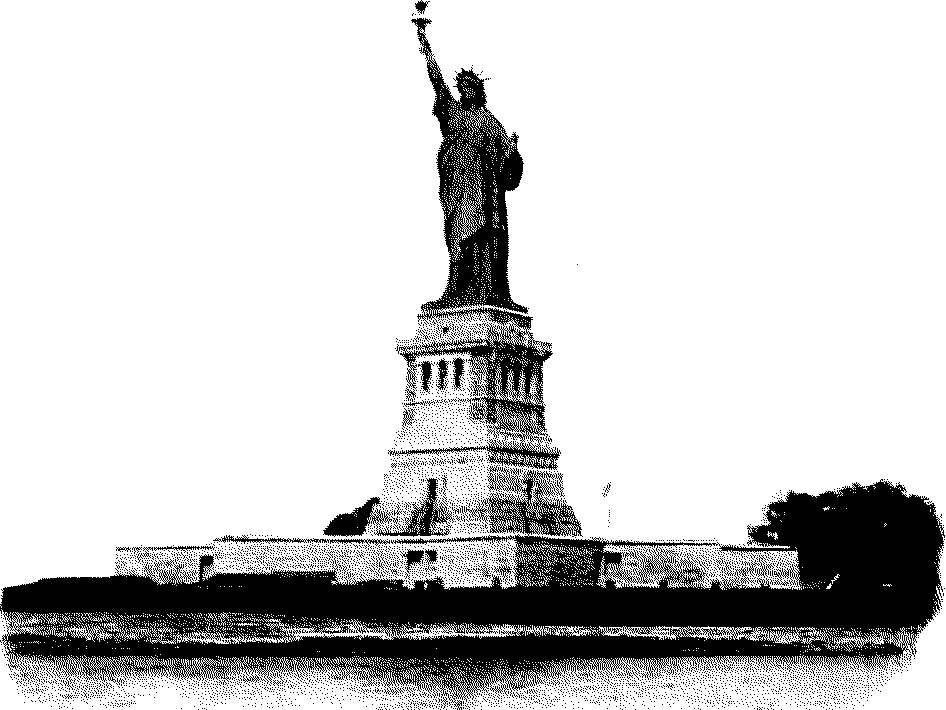
\includegraphics[width=6cm]{14_2019_Shadura1.jpg}
  %\caption{Statue of Liberty}	
  \label{fig1}
\end{figure}
\end{center}

Very soon though, during the first world war, passports returned as a temporary measure. Nothing is as permanent as temporary measures, it is often said. Passports were here to stay, and by 1947 getting rid of them has become a distant dream.

Software copyrights are in a way similar. Initially, software was not protected by copyrights or similar laws at all. In particular, in the US, prior to 1974, object code wasn't copyrightable due to lack of creativity while the consensus on the source code was that it was not copyrightable, because computer programs could be considered ideas, procedures, methods, systems, and processes.

In fact, quite a lot of software was distributed as source code: 
\begin{center}
\begin{figure}[h!]
  \centering
  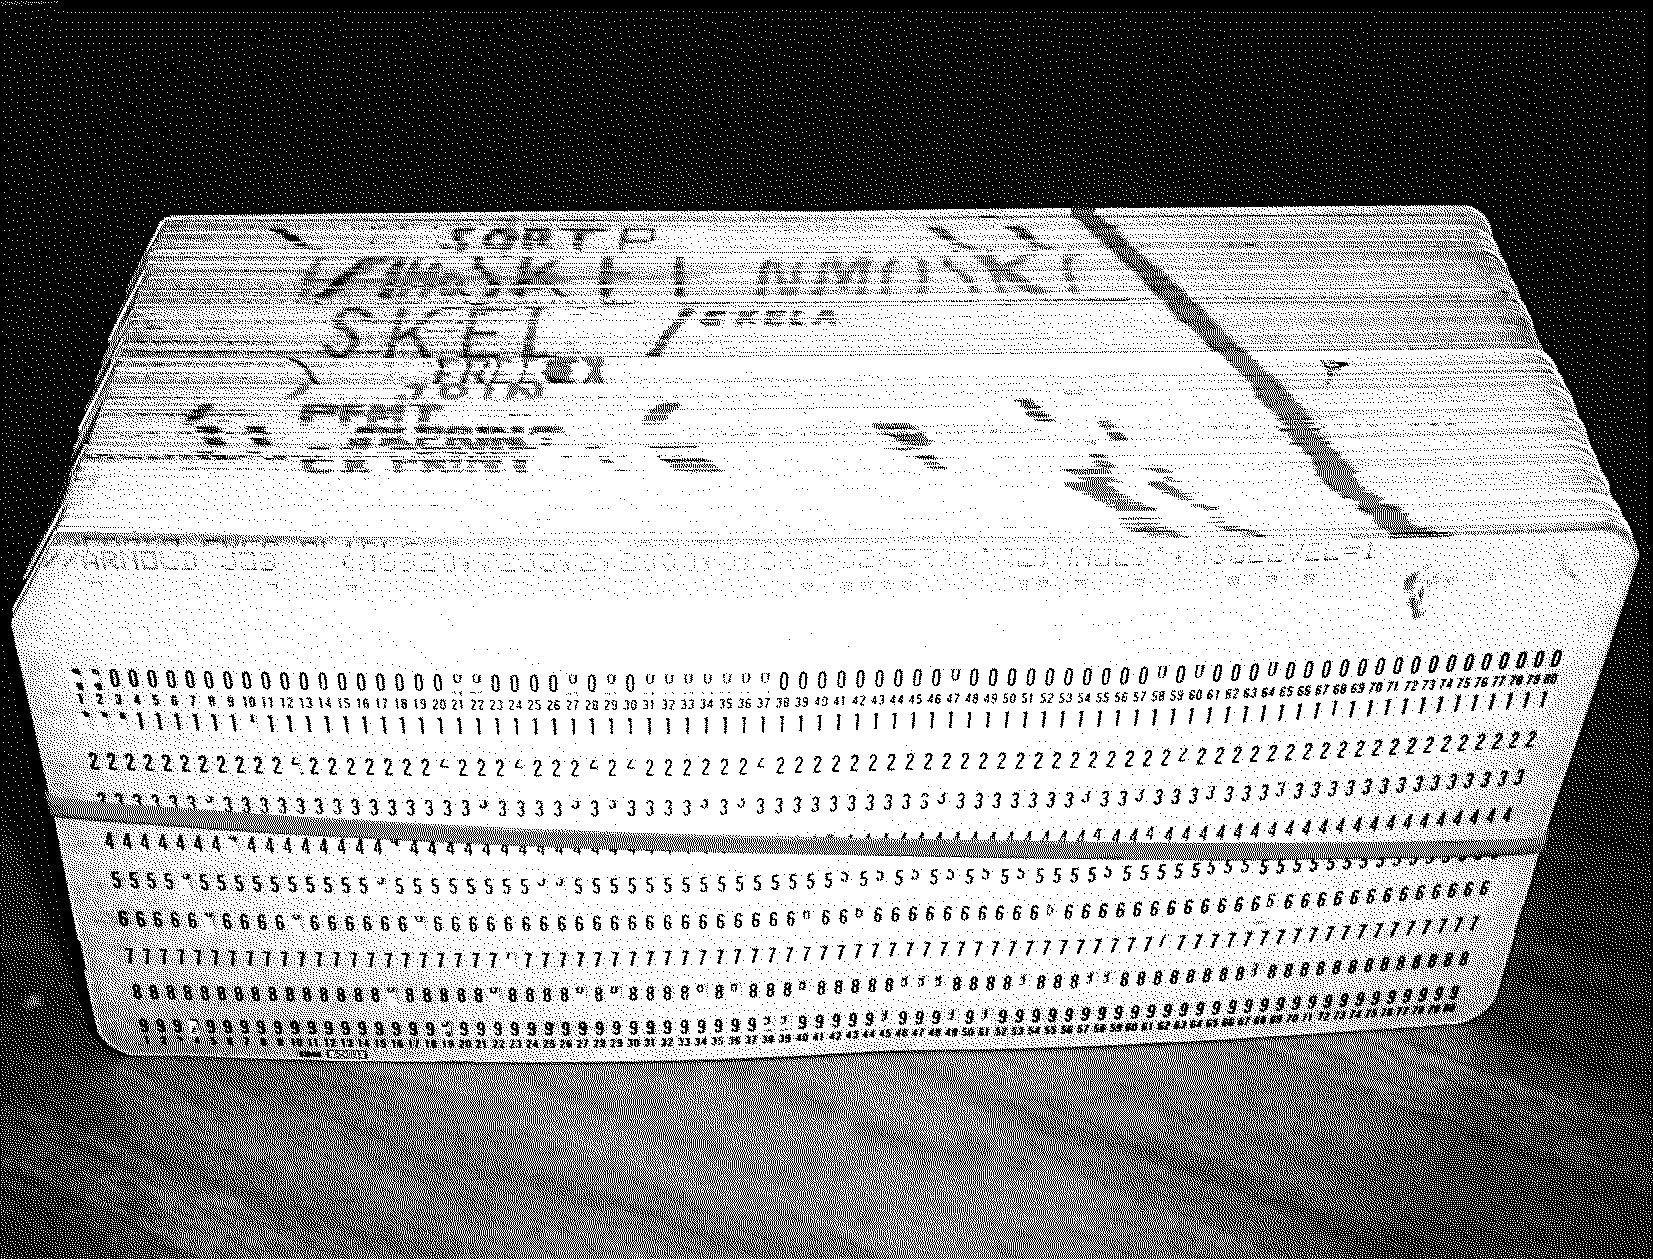
\includegraphics[width=7cm]{14_2019_Shadura2.jpg}
  
  \label{fig2}
\end{figure}
\end{center}

However, the Commission on New Technological Uses of Copyrighted Works formed in 1974, has decided that <<computer programs, to the extent that they embody an author's original creation, are proper subject matter of copyright>>. This decision followed by the US Copyright Act of 1976 giving computer programs the status of <<literary works>>.

This development has made a lot of people unhappy. One of the unhappy people was Richard Stallman. Richard Stallman was one of the people who worked at the MIT artificial intelligence lab on one of these:

\begin{center}
\begin{figure}[h!]
  \centering
  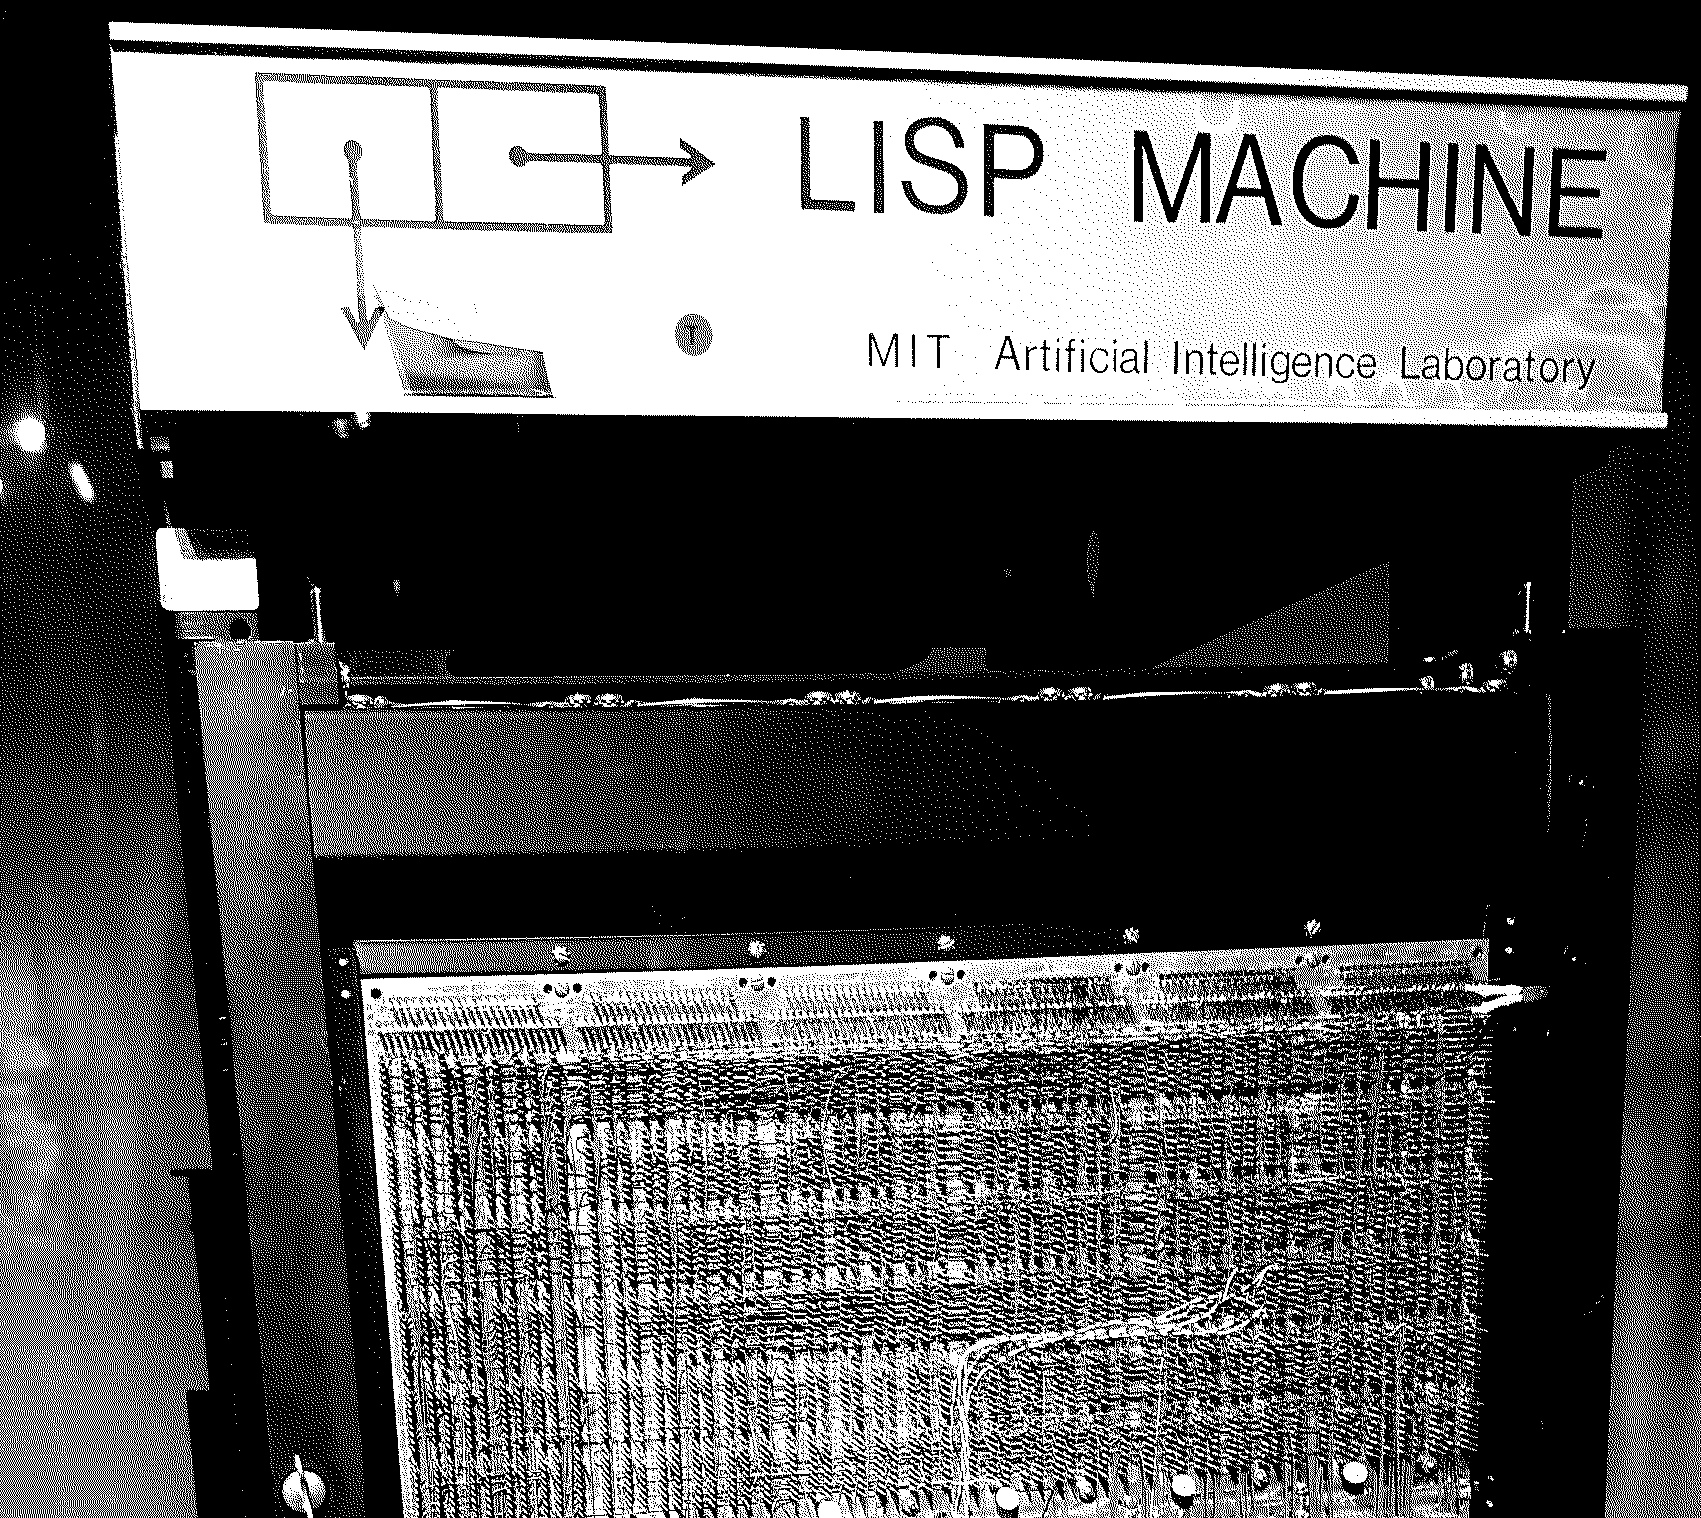
\includegraphics[width=6cm]{14_2019_Shadura3.jpg}
  
  \label{fig3}
\end{figure}
\end{center}

At MIT AI lab, there was the culture of sharing, part of the so-called hacker ethic:

\begin{quotation}
\ldots{}You would devise your own solution --- or <<hack.>> And then you'd share it with everyone else. Because\ldots{} why not?

\end{quotation}

One day, Richard Stallman was very unhappy about the new laser printer. The printer, just as the old one, was jamming paper. When this happened before, Stallman modified the printer driver to detect the jam and report it, but when he attempted to do this for the new printer, his request for the source code was rejected.

\begin{center}
\begin{figure}[h!]
  \centering
  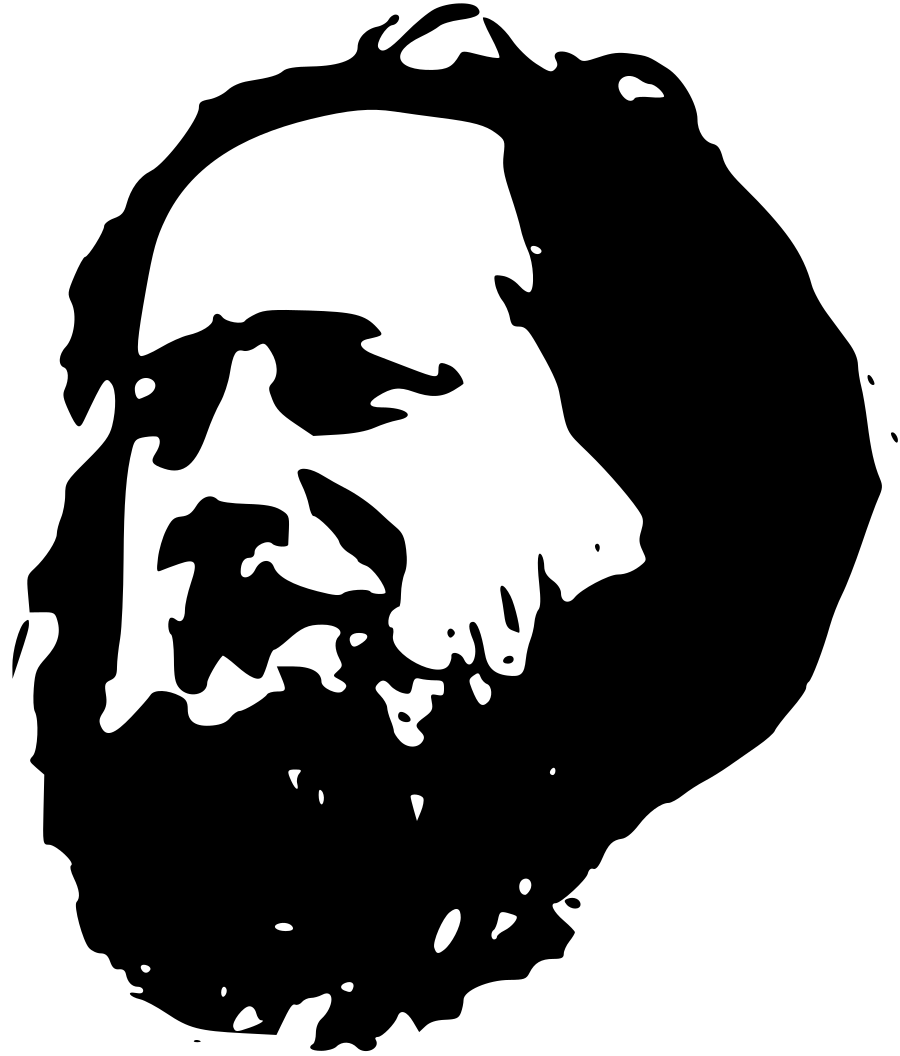
\includegraphics[width=4cm]{14_2019_Shadura4.png}
  
  \label{fig4}
\end{figure}
\end{center}

In 1983, Stallman, fed up with software coming with restrictions attached, publishes GNU Manifesto, a document which set out a plan to develop a free operating system, GNU. Several years later, he's published a detailed definition of that freedom:

\begin{enumerate}
  \item The freedom to run the program as you wish, for any purpose.
  \item The freedom to study how the program works and change it.
  \item The freedom to redistribute copies so you can help others.
  \item The freedom to distribute copies of your modified versions to others.
\end{enumerate}

Software providing those four freedoms to its users is called free software. The GNU operating system was meant to be fully free software. To protect software freedom, Stallman wrote a new license in 1989, the General Public License. This license uses the legal framework of copyright to guarantee the users can enjoy the four freedoms. It also guarantees all derivative works use the same license, and no restrictions can be added on top of the license; it explicitly makes them void.

By 1991, the GNU project completed the development of all major components of the operating system but the kernel, a core part of the operating system that manages the hardware, resources, devices\ldots{} basically, has complete control over everything in the system.

On 25 August 1991, Linus Torvalds posted the following to comp.os. minix, a newsgroup on Usenet:

\begin{quotation}
I'm doing a (free) operating system (just a hobby, won't be big and professional like gnu)

\end{quotation}

Linus has been developing the new OS  —  Linux  —  since April that year. The GNU Project soon embraced Linux, since own kernel, Hurd, was incomplete and unavailable, and another free OS, the Berkeley Software Distribution was involved in a lawsuit, and its status was unclear at the time.

In 1993, Ian Murdock announces the Debian project, which aims to build an operating system built on GNU and Linux. In Linux world, that's what a distribution is.

In many software projects, the project's creator leads the project since its inception for a long period of time. This was not the case with Debian. Instead of being a Benevolent Dictator for Life, Ian first delegated rôles to other members of the community, and then stepped down in 1996, with Bruce Perens replacing him.

\begin{quotation}
Rather than being developed by one isolated individual or group, as other distributions of Linux have been developed in the past, Debian is being developed openly in the spirit of Linux and GNU.  ---  Ian Murdock, the Debian Manifesto, 1994

\end{quotation}

What makes Debian different from other distributions? First of all, by some metrics, it's the biggest one. It supports the most different types of hardware architectures, and it has the most software packages included (if we don't count Ubuntu, which builds on top of Debian and adds software of their own). Second, it is run by a community of independent developers all around the world: there's no single company behind it, so interests of the projects can't be compromised by the interests of the company shareholders. Third, the project is built on an open democratic governance model.

\begin{quotation}

\ldots{} if you remove the community from open source software, it's just software (2003)

The Debian design process is open to ensure that the system is of the highest quality and that it reflects the needs of the user community.

\end{quotation}

Finally, the project pays a lot of attention to guarding the software freedom.

Soon after Bruce Perens became the project leader, he has proposed a document which summarised the moral principles of the Debian project, supplementing the initial \emph{Debian Manifesto} written by Murdock. The creation of the document was triggered by a discussion at Red Hat, a company behind a commercial Red Hat Linux distribution, where the idea for Red Hat to provide a set of guarantees it would always be committed to the ideals of free software was met with resistance. The document, ratified on 5 July 1997, was called the Debian Social Contact.

\begin{enumerate}
  \item Debian will remain 100\% free
  \item We will give back to the free software community
  \item We will not hide problems
  \item Our priorities are our users and free software
  \item Works that do not meet our free software standards
\end{enumerate}

DFSG:

\begin{enumerate}
  \item Free Redistribution
  \item Source Code
  \item Derived Works
  \item Integrity of The Author>>s Source Code
  \item No Discrimination Against Persons or Groups
  \item No Discrimination Against Fields of Endeavour
  \item Distribution of License
  \item License Must Not Be Specific to Debian
  \item License Must Not Contaminate Other Software
\end{enumerate}

These criteria while similar to the Four Freedoms, are more practical since they are easier to test against: it can be difficult to determine exactly how the terms of a specific license map to the user>>s freedoms. The Debian free software guidelines, on the contrary are more atomic, so it is easier to verify whether or not the license follows them. However, they define the same set of the licenses and the FSF>>s Four Freedoms.

In early 1998, a company called Netscape was about to release the source code of their browser under a free software license. A group of people, including Christine Peterson of Foresight Institute, met to discuss the promotion of free software to businesses, including Netscape.

\begin{center}
\begin{figure}[h!]
  \centering
  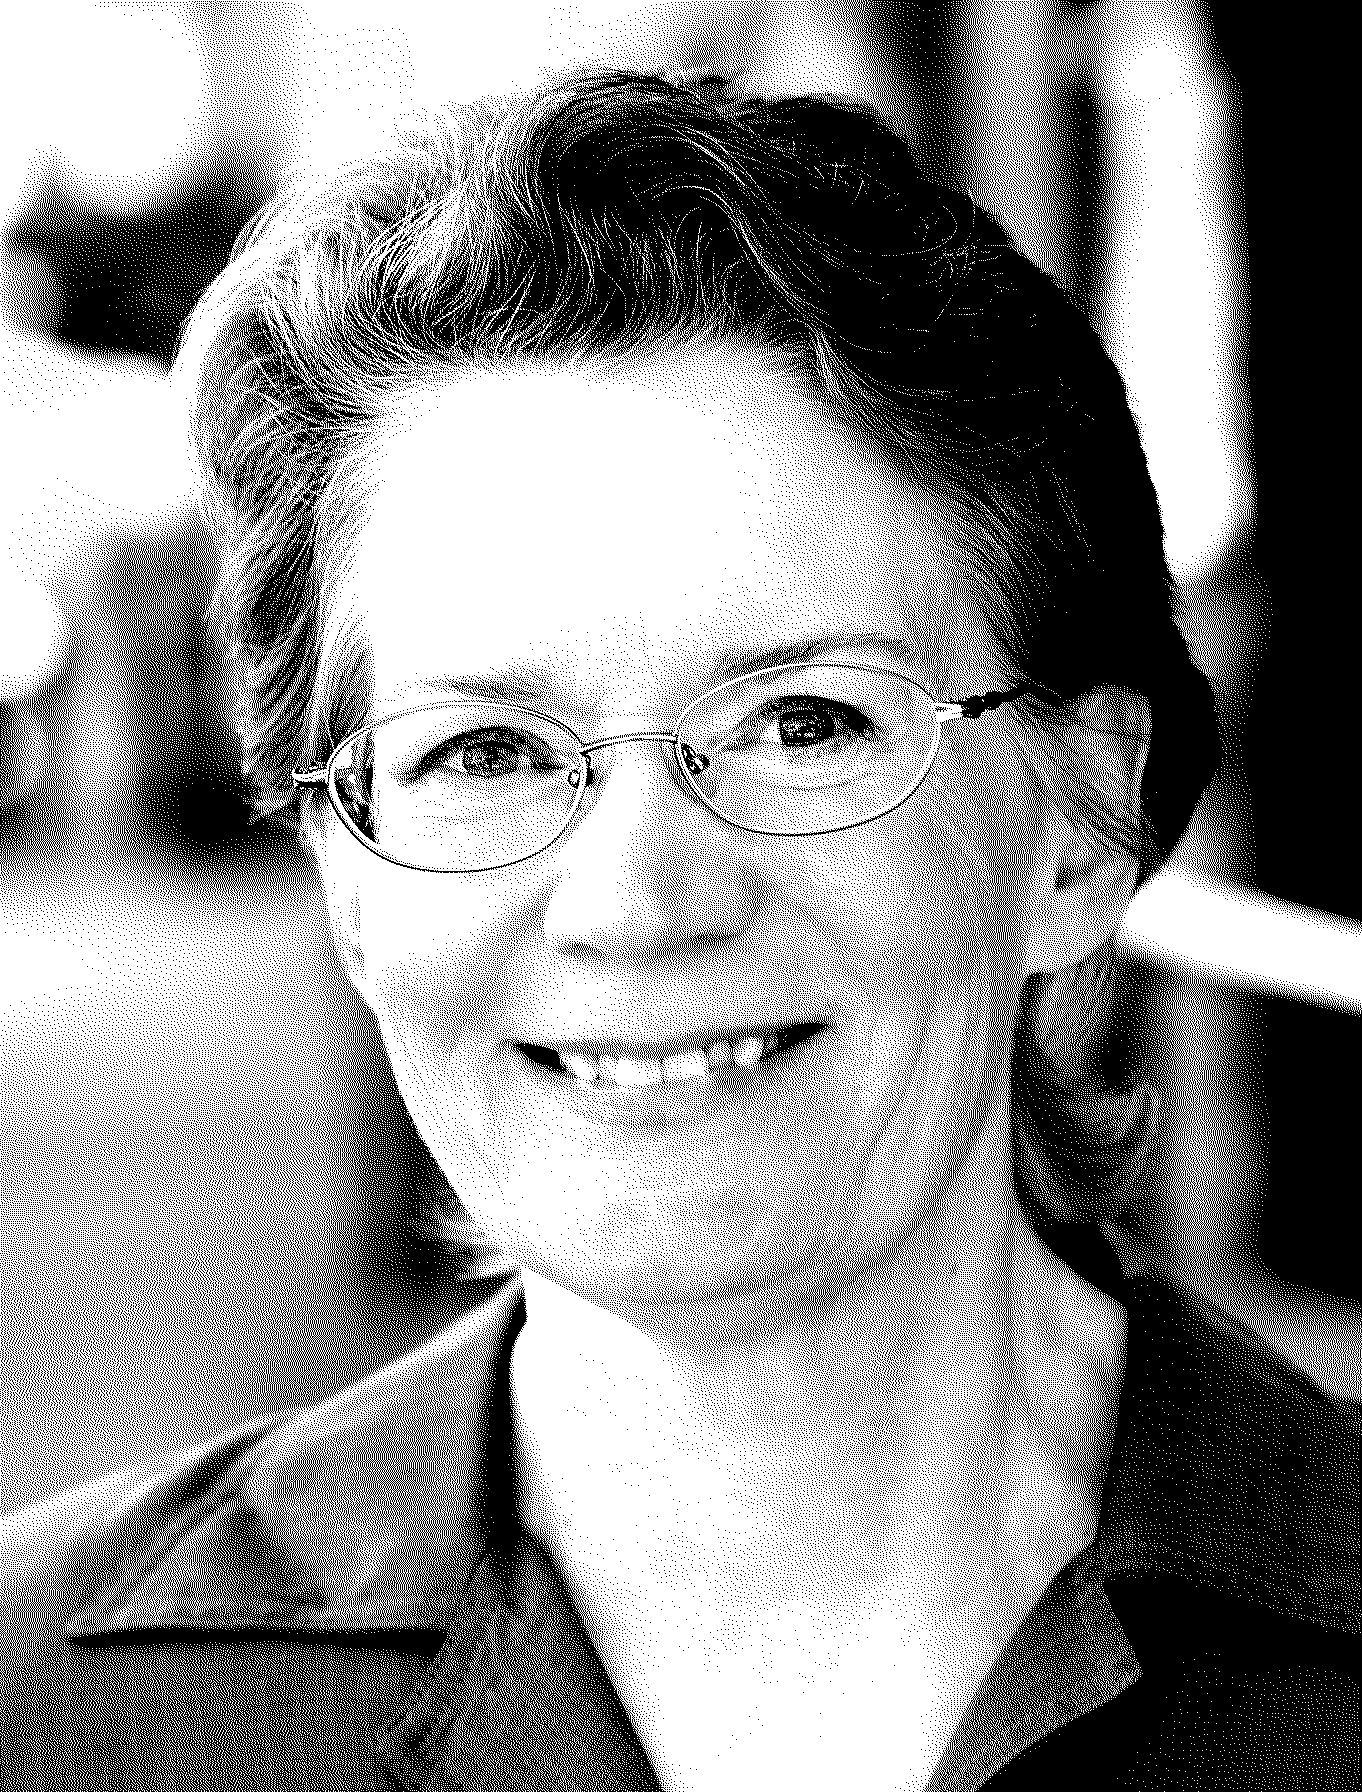
\includegraphics[width=4.5cm]{14_2019_Shadura5.jpg}
  
  \label{fig5}
\end{figure}
\end{center}

One of the topics was a new term to use because \emph{free software} was a bit confusing to people not knowing about it: they would assume it was about the price. Usually, we say \emph{We mean free as in freedom, not free as in beer}, but a new, clearer term was necessary.

During one of the meetings Christine came up with \emph{open source}, which, while not idea, seemed to her as good enough. After having discussed it with other group members, the term was eventually accepted. A new movement was started, with Bruce Perens joining the effort and establishing an organisation, the Open Source Initiative. Bruce Perens wrote a document called \emph{Open Source Definition}, based on the DFSG with references to Debian removed or replaced:

\begin{enumerate}
  \item Free Redistribution
  \item Source Code
  \item Derived Works
  \item Integrity of The Author>>s Source Code
  \item No Discrimination Against Persons or Groups
  \item No Discrimination Against Fields of Endeavour
  \item Distribution of License
  \item License Must Not Be Specific to \st{Debian} \emph{a Product}
  \item License Must Not \st{Contaminate} \emph{Restrict} Other Software
  \item \emph{License Must Be Technology-Neutral}
\end{enumerate}

Free software definition:

\begin{itemize}
  \item Promotes the philosophy of freedom
  \item Focuses on the rights of the user to use, study, modify, copy and redistribute the program for any purpose
\end{itemize}

Open source definition:

\begin{itemize}
  \item Promotes the practical values of software freedom and open development methodology
  \item Focuses on the availability of the source code and unrestricted development
\end{itemize}

Both definition require allowing commercial use.

Despite the differences, both concepts define nearly the same set of software licenses. For all practical purposes, free software and open source software mean the same thing. The main difference is in the way they define this same thing.

\begin{center}
\begin{figure}[h!]
  \centering
  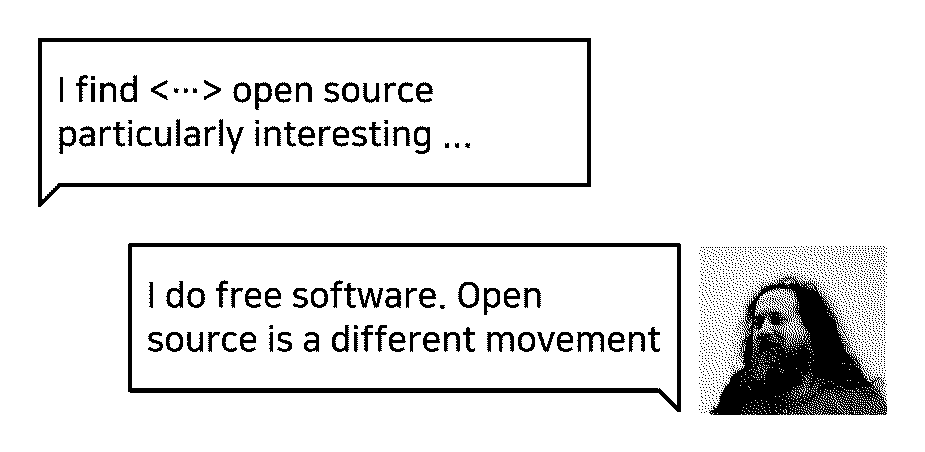
\includegraphics[width=6cm]{14_2019_Shadura6.png}
  
  \label{fig4}
\end{figure}
\end{center}


However, having initially praised open source, Richard Stallman later decided to reject it. He says the campaign for open source gets too pragmatic and doesn>>'t promote the moral principles of free software. For free software campaigners, the movement's ethical and social values are very important, and some, including Stallman, think all software should be free.

On the other hand, a lot of people love free software, but think that idea is way too radical. They accept the reality that a lot of software out there is non-free, but we can convince businesses to move to free software as much as possible. For those purposes, the concept of open source is often more useful, since it avoids telling people they're doing immoral things.

There's a concern Stallman also mentions, that both terms have ways to be misunderstood, but the \emph{wrong} meaning of open source doesn't say anything about freedom. In practice, that leads to situations, when companies promote their software calling it open source, while not providing the source code under a free software license. One of the companies which used to do that was Microsoft in 2000s, which released software under a license which basically only allowed to look at it  ---  provided you immediately forgot what you learnt from it. There more tricky situations, though.

JSON license:

\begin{itemize}
  \item The Software shall be used for Good, not Evil.
\end{itemize}

This is discrimination against fields of endeavour: you are not \linebreak allowed to do evil with this software. The author of the license, Douglas Crockford, who has also wrote JSMin, refused to change the license when was asked to. He has, however, granted <<IBM, its customers, partners, and minions>> permission <<to use JSLint for evil>>.

Do No Harm License:

\begin{quotation}
\ldots{}based on the BSD 3-clause license, but with specific exclusions for using licensed code to promote or profit from: violence, hate and division, environmental destruction, abuse of human rights, the destruction of people's physical and mental health\ldots{}

\end{quotation}

The annotated version of the open source definition states:

\begin{quotation}
We want commercial users to join our community, not feel excluded from it.

\end{quotation}


\end{document}
